% Options for packages loaded elsewhere
\PassOptionsToPackage{unicode}{hyperref}
\PassOptionsToPackage{hyphens}{url}
%
\documentclass[
]{book}
\title{Portfólio Gabriel Maciel}
\author{Gabriel Maciel}
\date{2022-03-03}

\usepackage{amsmath,amssymb}
\usepackage{lmodern}
\usepackage{iftex}
\ifPDFTeX
  \usepackage[T1]{fontenc}
  \usepackage[utf8]{inputenc}
  \usepackage{textcomp} % provide euro and other symbols
\else % if luatex or xetex
  \usepackage{unicode-math}
  \defaultfontfeatures{Scale=MatchLowercase}
  \defaultfontfeatures[\rmfamily]{Ligatures=TeX,Scale=1}
\fi
% Use upquote if available, for straight quotes in verbatim environments
\IfFileExists{upquote.sty}{\usepackage{upquote}}{}
\IfFileExists{microtype.sty}{% use microtype if available
  \usepackage[]{microtype}
  \UseMicrotypeSet[protrusion]{basicmath} % disable protrusion for tt fonts
}{}
\makeatletter
\@ifundefined{KOMAClassName}{% if non-KOMA class
  \IfFileExists{parskip.sty}{%
    \usepackage{parskip}
  }{% else
    \setlength{\parindent}{0pt}
    \setlength{\parskip}{6pt plus 2pt minus 1pt}}
}{% if KOMA class
  \KOMAoptions{parskip=half}}
\makeatother
\usepackage{xcolor}
\IfFileExists{xurl.sty}{\usepackage{xurl}}{} % add URL line breaks if available
\IfFileExists{bookmark.sty}{\usepackage{bookmark}}{\usepackage{hyperref}}
\hypersetup{
  pdftitle={Portfólio Gabriel Maciel},
  pdfauthor={Gabriel Maciel},
  hidelinks,
  pdfcreator={LaTeX via pandoc}}
\urlstyle{same} % disable monospaced font for URLs
\usepackage{longtable,booktabs,array}
\usepackage{calc} % for calculating minipage widths
% Correct order of tables after \paragraph or \subparagraph
\usepackage{etoolbox}
\makeatletter
\patchcmd\longtable{\par}{\if@noskipsec\mbox{}\fi\par}{}{}
\makeatother
% Allow footnotes in longtable head/foot
\IfFileExists{footnotehyper.sty}{\usepackage{footnotehyper}}{\usepackage{footnote}}
\makesavenoteenv{longtable}
\usepackage{graphicx}
\makeatletter
\def\maxwidth{\ifdim\Gin@nat@width>\linewidth\linewidth\else\Gin@nat@width\fi}
\def\maxheight{\ifdim\Gin@nat@height>\textheight\textheight\else\Gin@nat@height\fi}
\makeatother
% Scale images if necessary, so that they will not overflow the page
% margins by default, and it is still possible to overwrite the defaults
% using explicit options in \includegraphics[width, height, ...]{}
\setkeys{Gin}{width=\maxwidth,height=\maxheight,keepaspectratio}
% Set default figure placement to htbp
\makeatletter
\def\fps@figure{htbp}
\makeatother
\setlength{\emergencystretch}{3em} % prevent overfull lines
\providecommand{\tightlist}{%
  \setlength{\itemsep}{0pt}\setlength{\parskip}{0pt}}
\setcounter{secnumdepth}{5}
\usepackage{booktabs}
\ifLuaTeX
  \usepackage{selnolig}  % disable illegal ligatures
\fi
\usepackage[]{natbib}
\bibliographystyle{plainnat}

\begin{document}
\maketitle

{
\setcounter{tocdepth}{1}
\tableofcontents
}
\hypertarget{sobre-mim}{%
\chapter{Sobre Mim}\label{sobre-mim}}

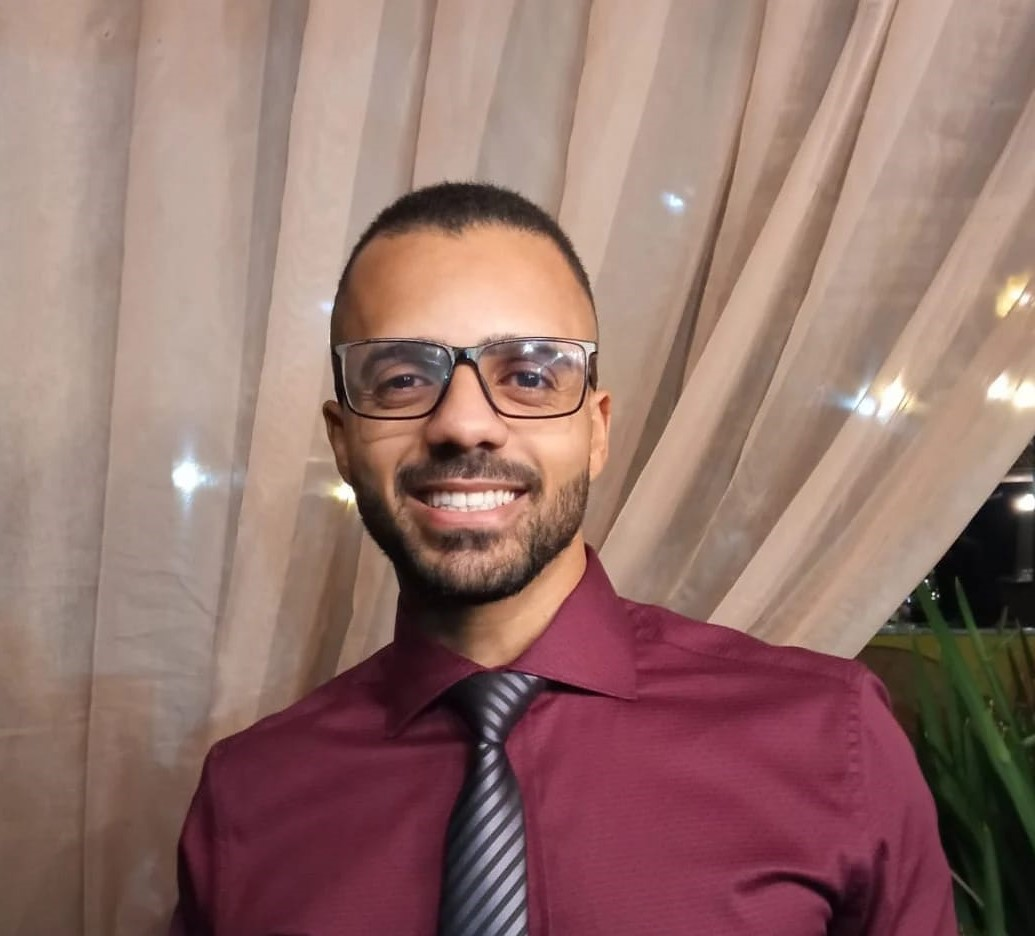
\includegraphics[width=3.125in,height=\textheight]{C:/Users/gabri/Documents/Projetos/Portfolio/Gabriel Maciel.jpeg}

Olá, bem vindo ao meu portfólio de ciência de dados, nele eu vou falar um pouco sobre minha relação com estatística e ciência de dados, mostrar minhas habilidades e experiências profissionais.

E-mail: \href{mailto:gabrielmacieldias@hotmail.com}{\nolinkurl{gabrielmacieldias@hotmail.com}}

Celular: (31) 98905-9541

\hypertarget{curiosidades}{%
\section{Curiosidades}\label{curiosidades}}

Meu nome é Gabriel Maciel Dias, tenho 23 anos e moro na cidade de Belo Horizonte.

Como todo aluno bom em matemática no ensino médio eu me imaginava fazendo faculdade de engenharia, entretanto acabei conhecendo o curso de Estatística na mostra de profissões da UFMG, nela me mostraram um pouco de como a estatística está presente em nossa vida.

Em 2016 fiz o Enem e em 2017 entrei no curso de Estatística, desde então me apaixonei pela área e agora luto diariamente para tentar aprender mais e mais todos os dias.

\hypertarget{formauxe7uxe3o}{%
\section{Formação}\label{formauxe7uxe3o}}

Bacharel em Estatística na Universidade Federal de Minas Gerais (UFMG) 2017 - 2021

\hypertarget{experiuxeancia-profissional}{%
\section{Experiência Profissional}\label{experiuxeancia-profissional}}

Desde que comecei na graduação passei por alguns estágios em áreas diferentes. Atualmente trabalho como Assistente de Crédito no Banco Semear e também como cientista de dados na startup Sua Rua.

\hypertarget{estagiuxe1rio-hospital-odilon-behrens---abril2018-uxe0-outubro2018}{%
\subsection{Estagiário Hospital Odilon Behrens - Abril/2018 à Outubro/2018}\label{estagiuxe1rio-hospital-odilon-behrens---abril2018-uxe0-outubro2018}}

Responsável pela confecção de relatórios mensais, além do atendimento de demanda de dados, fazendo a retirada deles em um banco específico do hospital. Durante esse período de trabalho elaborei alguns códigos na linguagem de programação R com o objetivo de aperfeiçoar relatórios e análises de dados.

\hypertarget{estagiuxe1rio-no-setor-de-estatuxedstica-da-reitoria-da-ufmg---novembro2018-uxe0-junho2020}{%
\subsection{Estagiário no Setor de Estatística da Reitoria da UFMG - Novembro/2018 à Junho/2020}\label{estagiuxe1rio-no-setor-de-estatuxedstica-da-reitoria-da-ufmg---novembro2018-uxe0-junho2020}}

Responsável pela elaboração de relatórios com análises descritivas e modelos de regressão, com finalidade de analisar o perfil e o desempenho dos estudantes da UFMG e divulgar o resultado em sites da universidade. Além disso, eram atendidos demandas de dados feitas por funcionários da universidade. Neste período os relatórios foram feitos usando o software R em conjunto com o R Markdown, Latex e excel.

\hypertarget{estagiuxe1rio-de-cruxe9dito-no-banco-de-desenvolvimento-de-minas-gerais-julho2020-uxe0-dezembro2020}{%
\subsection{Estagiário de Crédito no Banco de Desenvolvimento de Minas Gerais -- Julho/2020 à Dezembro/2020}\label{estagiuxe1rio-de-cruxe9dito-no-banco-de-desenvolvimento-de-minas-gerais-julho2020-uxe0-dezembro2020}}

Responsável pela conferência de planilhas de classificação de risco e criação de programa em R para automatizar determinadas conferências de dados. Além disso, também faço trabalhos com simulações (em Python e R) de carteiras de crédito para prever possíveis perdas.

\hypertarget{estagiuxe1rio-de-cruxe9dito-no-banco-bs2-janeiro2021-uxe0-agosto2021}{%
\subsection{Estagiário de Crédito no Banco BS2 -- Janeiro/2021 à Agosto/2021}\label{estagiuxe1rio-de-cruxe9dito-no-banco-bs2-janeiro2021-uxe0-agosto2021}}

Responsável pelos atendimentos de ordens de serviço relacionado a dúvidas sobre análise de crédito além verificar como está o andamento de uma solicitação de crédito dentro do sistema do banco. Além disso, também trabalho na confecção de relatórios Backtest em R em conjunto com R Markdown com base de dados retiradas do SQL Server para verificar como a esteira de crédito está funcionando e se ela está tomando boas decisões de previsão.

\hypertarget{assistente-de-cruxe9dito-no-banco-semear---setembro2021---atualmente}{%
\subsection{Assistente de Crédito no Banco Semear - Setembro/2021 - Atualmente}\label{assistente-de-cruxe9dito-no-banco-semear---setembro2021---atualmente}}

Responsável por criação de dashboards para tomada de decisões usando dados de carteira e esteira de crédito. Participo de comitês de crédito, reuniões com fornecedores de dados e de modelos e reuniões com lojistas do banco.
Faço também rateio e pagamento de fornecedores, estudo de base de dados para pré aprovado, bem como sugestões de análises que podem ajudar na resolução de problemas de negócio.
Todas as análises faço através do software R em conjunto com o Shiny e Excel.

\hypertarget{cientista-de-dados-na-sua-rua---agosto2021---atualmente}{%
\subsection{Cientista de Dados na Sua Rua - Agosto/2021 - Atualmente}\label{cientista-de-dados-na-sua-rua---agosto2021---atualmente}}

Nessa startup trabalho com construção de modelos de dados geográficos, trabalhando com R e QGis, além disso atuo coletando dados e criando robôs para fazer Web Scrapping.

\hypertarget{habilidades}{%
\section{Habilidades}\label{habilidades}}

Programação avançada em R

Criação de relatórios com R Markdown

Criação de Dashboards com Shiny

Inglês intermediário

Pacote Office

\hypertarget{projetos}{%
\chapter{Projetos}\label{projetos}}

\hypertarget{banco-iris}{%
\section{Banco Iris}\label{banco-iris}}

\hypertarget{outro-banco}{%
\section{Outro banco}\label{outro-banco}}

  \bibliography{book.bib,packages.bib}

\end{document}
